\chapter{Grundlagen}
\label{background}

Alle Quellen hier referenzieren!

%- Allgemeine Wissensgrundlagen des Fachgebiets
%- Spezielle Grundlagen, die für das Verständnis erforderlich sind
%- Rahmenbedingungen für die Arbeit
%- Ausführungen zum Stand des Wissens / der Technik
%Als Leitprinzip gilt: Nur Informationen erwähnen, die
%- später benötigt werden,
%- notwendig sind, um die Arbeit oder ihre Motivation zu verstehen
%Das heißt insbesondere,
%- keine Inhalte aus Lehrbüchern, außer
%- diese werden benötigt, um Problemstellung oder Lösungsweg zu definieren.

%Was sind Pen&Paper spiele?
%Was tun die Spieler?
%Was tut der Spielleiter?


\section{Pen\&Paper Spiele}
\label{sec:PenPaperSpiele}

\begin{itemize}
	\item Kurze Erklärung wie so etwas abläuft
	\item Übersicht über bekannte PnP Spiele, was ist an D\&D besonders?
	\item \textit{[Abgrenzung zu normalen RPGs]} NEIN, da in \ref{sec:DigitaleRollenspiele}
\end{itemize}


\subsection{Spielleiter}
\label{sec:Spielleiter}
Beschreibung der Tätigkeiten und Funktion von Spielleitern beim PnP\newline
Abdecken von:
\begin{itemize}
	\item Konzeption und Umsetzung eines Abenteuers ('offline' vor der Spielrunde)
	\item Durchführen des Spieles ('online' währen der Runde mit dem Spielern zusammen)
\end{itemize}
Der Spielleiter hat bei einem PnP Rollenspiel die Aufgabe eine Geschichte für die Spielrunde zu erdenken und die Teilnehmer während des Verlaufes anzuleiten. Im Vorfeld der Spielrunde konzipiert der Spielleiter dafür eine Ausarbeitung eines Abenteuers. Meist werden hierfür Kerncharaktere und wichtige Entscheidungspunkte / Szenen ausgearbeitet, während sich der genaue Verlauf des Abenteuers beim Spielen ergibt. \ref{fig:storyflow_pnp} zeigt, wie auf mehreren Ideen des Spielleiters durch Einflussnahme und Interaktion der Spieler eine Geschichte wird. Um diese Entwicklung zu ermöglichen muss der Spielleiter verschiedene Funktionen erfüllen.\newline
\cite{Arinbjarnar} nennt drei verschiedene Kernaufgaben des Spielleiters: \emph{Storyteller}, \emph{Actor} und \emph{Judge}. Zum einen ist es die Aufgabe des Spielleiters die Geschichte aus objektiver Sicht zu erzählen und die Handlung mit den Spielern voranzutreiben. Gleichzeitig nimmt er jedoch auch die Rolle und den Standpunkt aller NSCs ein und vermittelt zwischen ihnen und den Spielern. Als letzte Aufgabe achtet der Spielleiter auf die Einhaltung aller Regeln und trifft Entscheidungen falls es zu Unstimmigkeiten kommt.
\begin{figure}
	\centering
		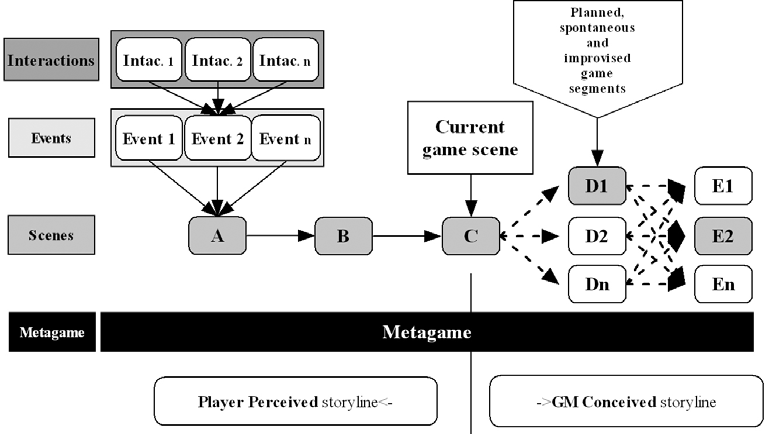
\includegraphics[width=1.00\textwidth]{media/storyflow_pnp.png}
	\caption{Entwicklung einer Geschichte nach \cite{Tychsen2006a}}
	\label{fig:storyflow_pnp}
\end{figure}




\subsection{Spielermotivation}
\label{sec:Spielermotivation}

\begin{itemize}
	\item Hervorheben was die PnP Spieler wollen (nach Möglichkeit belegen: Paper, Foren, unsere Testspieler, Pathfinder Entwickler)
	
	\begin{itemize}
		\item Kreative Interaktive Geschichte
		\item Soziale Komponente
		\item 'Gemeinsam Abenteuer erleben'
	\end{itemize}
\end{itemize}


\section{Digitale Rollenspiele}
\label{sec:DigitaleRollenspiele}

Beschreibung eines Standard Pc-Rollenspiels mit Mechaniken und Möglichkeiten\newline
Dient später der Abgrenzung zu unserem Prototypen
\begin{itemize}
	\item DSA Reihe
	\item D\&D Online
	\item Neverwinter Nights
	\item Elder Scrolls
	\item Baldurs Gate
	\item Icewind Dale
\end{itemize}
Besonders auf die D\&D basierten eingehen, den rest nur als Beispiele für andere Systeme.

\section{Bestehende Ansätze?}
\label{sec:BekannteAnsaetze}
Paper und Programme die unserem Thema ähneln, jeweils mit Abgrenzung warum sie die Frage nicht zufriedenstellend (oder wenigstens schlechter als wir) beantworten können
\begin{itemize}
	\item RPG Maker
	\item NWN
	\item GM-AI
	\item Tools die ähnliches leisten
\end{itemize}